\chapter{Contribution to the DREAM project} \label{app:dream}

As part of DREAM, I have been involved in various meetings, developed tools to automate tasks and contributed to a significant part of the software developed during the project.

\section{Software development}

WP6, composed of Plymouth and VUB, was responsible to develop the cognitive controller of the robot. I developed mostly alone the deliberative, expression and actuation and naoInterface subsystems. I also converted scripts provided by the therapist into steps the robot can follow and programmed a robot behaviour corresponding to each one of these steps.


\section{Tools}

In addition to the components developed to run the DREAM application, I created two tools to automate and simplify the use of the YARP middleware while conforming to the development standards imposed on the project.

\subsection{yarpGenerator}

The software development guidelines of DREAM imposed a specific structure for folders of new components developed with a number of constant part throughout the required 6 files. Additionally, adding or removing one port required changes in 5 files in more than 10 location. To ease this procedure, I proposed to add two new class: the yarpInterface and the yarpController. yarpInterface class exposes all the yarp output port required by the component to C++ function and integrates function asynchronously called when messages arrive on input ports. And the yarpController corresponds to a C++ only file where the code can be developed without reliance of YARP. This class (and others) can call functions from yarpInterface to send messages and be called by callbacks in yarpInterface to react to messages. The yarpGenerator is a tool generating automatically compilable code, complient with the development standards. Appendice B presents the techreport created to describe the tool.

\subsection{scriptManager}

The second tools aims at providing a graphical way to read and edit the xml files describing the scripts used in the therapies.

\cleartooddpage
\chapter{Teacher's Diary} \label{app:diary}
This appendix section present the daily report of the teacher's impressions and feeling when teaching the robot in the study in Chapter\ref{chap:tutoring}. It should be noted that among all the children supervised, many were special needs and as such have been removed from the result analysis. This also explains the difference of number between the children in the supervised condition (n=25) and in this diary (n=34).

%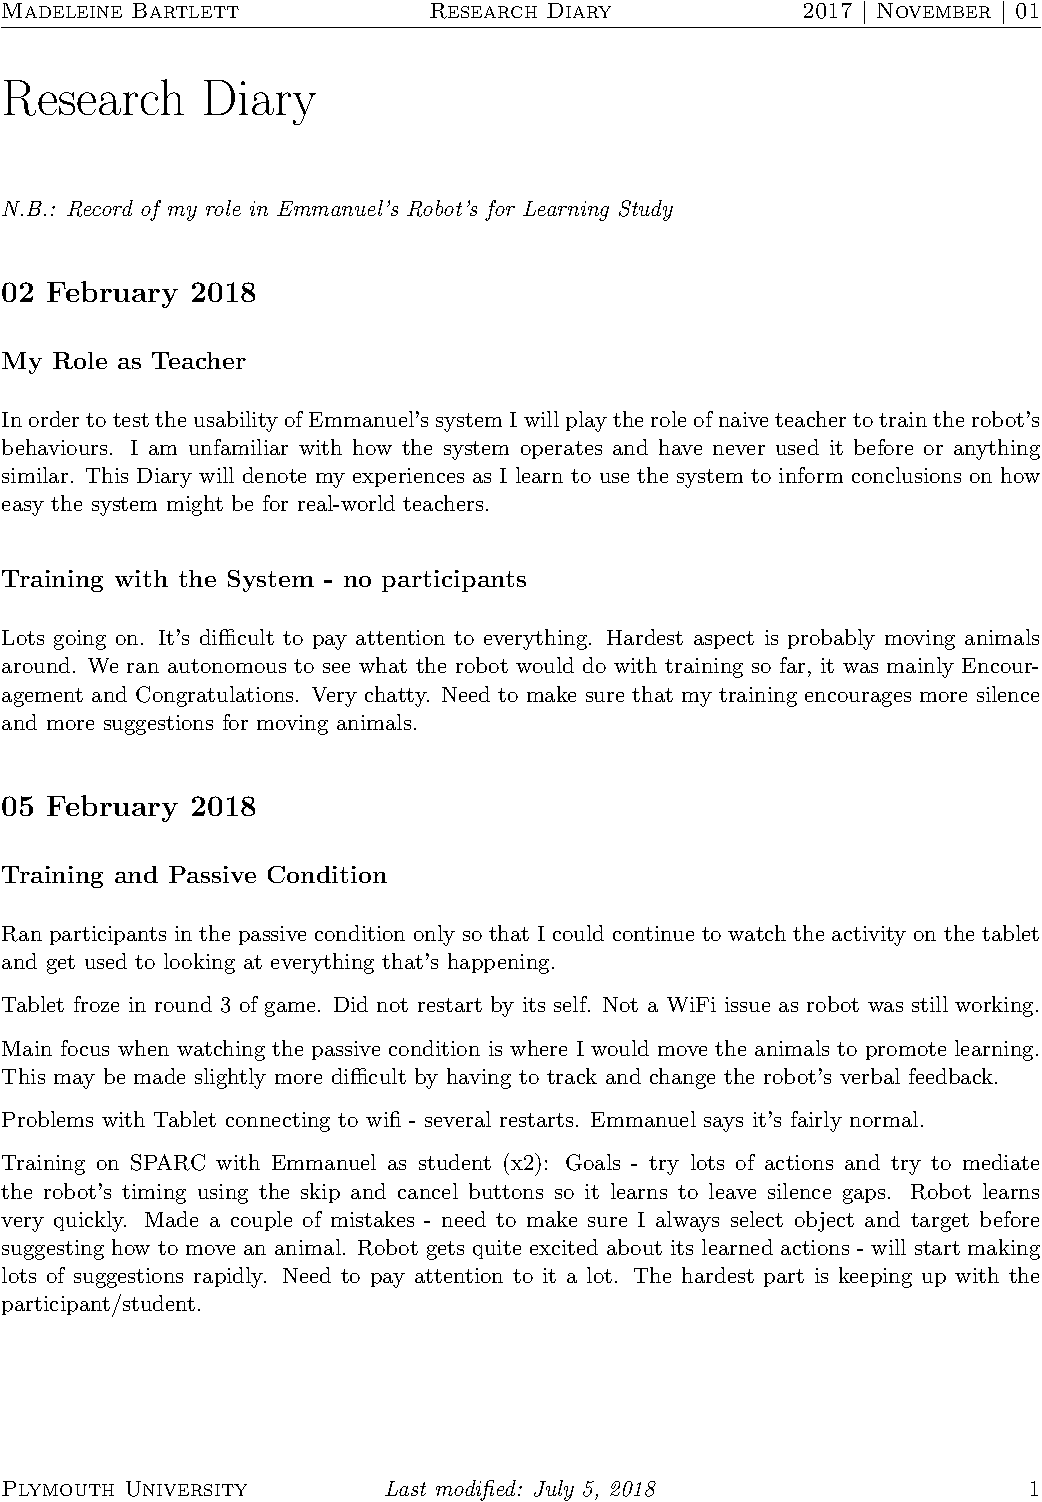
\includepdf[pages=1-14,pagecommand={},linktodoc=true]{appendices/research-diary.pdf}
\foreachpage{appendices/research-diary-crop.pdf}{%
	\newpage   
	\begingroup 
	\centering
	\includegraphics[
	page=\value{imagepage},
	width=\textwidth,  
	height=\textheight,
	keepaspectratio,
	]{appendices/research-diary-crop.pdf}%
	\newpage
	\endgroup
}